\documentclass[a4paper,11pt]{article}
\usepackage[utf8]{inputenc}
\usepackage{lastpage}
\usepackage{fancyhdr}
\usepackage[english]{babel}
\usepackage[a4paper,margin=1in]{geometry}
\usepackage{multirow}
\usepackage[table,xcdraw]{xcolor}
\usepackage{array}
\usepackage{amsmath}
\usepackage{amssymb}
\usepackage{relsize}
\usepackage{algorithm}
\usepackage{algpseudocode}
\usepackage{graphicx}
\usepackage[numbered,framed]{matlab-prettifier}
\usepackage{caption}

\captionsetup[table]{labelformat=empty}


\newcolumntype{L}[1]{>{\raggedright\let\newline\\\arraybackslash\hspace{0pt}}m{#1}}
\newcolumntype{C}[1]{>{\centering\let\newline\\\arraybackslash\hspace{0pt}}m{#1}}
\newcolumntype{R}[1]{>{\raggedleft\let\newline\\\arraybackslash\hspace{0pt}}m{#1}}

\def\margin#1#2{\list{}{\rightmargin#2\leftmargin#1}\item[]}
\let\endmargin=\endlist

\newcommand\tab[1][4mm]{\hspace*{#1}}
\newcommand{\norm}[1]{\left\lVert #1 \right\rVert}
\newcommand{\abs}[1]{\left\vert #1 \right\vert}

%-------------------------------------------------------------------------------
% HEADER & FOOTER
%-------------------------------------------------------------------------------

\pagestyle{fancy}
\fancyhf{}
\setlength\headheight{15pt}
\fancyhead[L]{ Numerical Analysis Assignment 2 }
\fancyhead[R]{Student ID: 100633486}
\fancyfoot[R]{Page \thepage\ of \pageref{LastPage}}


%-------------------------------------------------------------------------------
% TITLE PAGE
%-------------------------------------------------------------------------------

\begin{document}

\title{
	\Huge \textbf {Numerical Analysis}
    \\ [0.2cm]
	\LARGE Assignment 2, October 2017
    \\ [0.5cm]
    \hrule
}

\date{}

\author{
		\Large Kamyar Nazeri \\
		\large Student ID: 100633486 }

\maketitle

\newpage

\section*{Question 1.}
Matrix $A \in \mathbb{C}^{n\times n}$ is said to be \textit{strictly column diagonally dominant} if
\begin{equation}
\abs{a_{j,j}} > \sum_{\substack{i=1 \\ i\neq j}} \abs{a_{i,j}} \tab (j=1:n)
\end{equation}
\\
Prove that a strictly column diagonally dominant matrix is always nonsingular.
\\
\begin{margin}{0.5cm}{0.5cm}
	Suppose \textit{A} is singular, that is $det(A)=0$; then $A\mathbf{x}=0$ has non-trivial solution and there exists some non-zero vector $\mathbf{u}=(u_1, u_2,...,u_n)^T$ such that
	\begin{equation}
		A\mathbf{u}=0
	\end{equation}
	By taking the transpose of equation (2):
	\begin{equation}
		\mathbf{u}^T A^T=0
	\end{equation}
	
	Let \textit{k} be the index where
	
	\begin{equation*}
		u_k \geq u_i \tab \text{for all } \tab i=1,2...,n
	\end{equation*}
	
	From the \textit{k}-th row of equation (3), we obtain:
	
	\begin{equation}
		a_{(k,1)}u_1 + a_{(k,2)}u_2+...+a_{(k,k)}u_k+...+a_{(k,n)}u_n=0
	\end{equation}
	\begin{equation*}
		a_{(k,1)}u_1 + a_{(k,2)}u_2+...+a_{(k,n)}u_n=-a_{(k,k)}u_k
	\end{equation*}
	
	Hence:
	\begin{equation}
		\abs{a_{(k,k)}u_k}=\abs{\sum\limits_{i\neq k} a_{(k,i)}u_i }=\sum\limits_{i\neq k} \abs{a_{(k,i)}u_i}
	\end{equation}
	\begin{equation*}
		\abs{a_{(k,k)}}=\sum\limits_{i\neq k} \abs{a_{(k,i)}\frac{u_i}{u_k}}=\sum\limits_{i\neq k} \abs{a_{(k,i)}}\abs{\frac{u_i}{u_k}}
	\end{equation*}
	Since $\abs{\frac{u_i}{u_k}} \leq 1$ for every \textit{i}:
	
	\begin{equation}
		\abs{a_{(k,k)}} \leq \sum\limits_{i\neq k} \abs{a_{(k,i)}}
	\end{equation}
	
	Which is a contradiction with (1). Therefore assumption (2) is incorrect and $A\mathbf{x}=0$ has only trivial solution and \textit{A} is nonsingular.
\end{margin}

\newpage
\section*{Question 2.}
Write a program to construct a least-squares polynomial fitting certain data by distinct computational methods. In particular, find the least-squares polynomial of degree 11 (i.e., \textit{n} = 12) fitting \textit{m} = 50 points obtained by sampling the function $f(x) = cos(4x)$ at \textit{m} points uniformly spaced across the interval [0, 1]. That is, the programs should produce the 12 coefficients of the least-squares polynomial obtained by “solving” the over-determined linear system of equations.
\\\\
\noindent
\textbf{(a)}  Write a program to compute the coefficient matrix \textit{A} and the right-hand side vector $\mathbf{f}$.

\begin{lstlisting}[
style=Matlab-editor,
numbers=none,
frame=none,
xleftmargin=.2in
]
n = 12;                 % polynomial degree: (n-1)
m = 200;                % number of samples

x = linspace(0, 1, m);  % sample m points on the interval [0,1]
f = cos(4 * x)';        % evaluate function on sample points 
A = fliplr(vander(x));  % create the Vandermonde Matrix
A = A(:,1:n);           % get polynomials up to (n-1)
\end{lstlisting}
\noindent
\\\textbf{(b)} Modify your program from part (a) to compute the coefficients $\mathbf{c}^{(Chol)}$ obtained when solving the normal equations $A^TA\mathbf{c} = A^T\mathbf{f}$ by computing the Cholesky decomposition of $A^TA$

\begin{lstlisting}[
style=Matlab-editor,
numbers=none,
frame=none,
xleftmargin=.2in
]
% to solve the overdetermined system of equations Ac = f
% we calculate Cholesty decomposition of A'A and get A'A = LL'
% multiply both sides of the equation by A' => A'Ac=A'f 
% to solve for c: c_chol = inv(LL')A'f

[L] = chol(A'*A,'lower');   % lower triangular matrix L 
c_chol = L' \ (L \ (A'*f));
\end{lstlisting}

\noindent
\\\textbf{(c)} Modify your program from part (a) to compute the coefficients $\mathbf{c}^{(QR)}$ obtained using the QR decomposition of \textit{A}.

\begin{lstlisting}[
style=Matlab-editor,
numbers=none,
frame=none,
xleftmargin=.2in
]
% to solve the overdetermined system of equations Ac = f
% we calculate QR decomposition of A and get A = QR
% to solve for c: c_qr = inv(R)*Q'*f

[Q,R] = qr(A,0);            % reduced QR factors
c_qr = R\(Q'*f);            % inv(Q)=Q'
\end{lstlisting}

\noindent
\\\textbf{(d)} Modify your program from part (a) to compute the coefficients $\mathbf{c}^{(SVD)}$ obtained using the singular value decomposition of \textit{A}.

\begin{lstlisting}[
style=Matlab-editor,
numbers=none,
frame=none,
xleftmargin=.2in
]
% to solve the overdetermined system of equations Ac = f
% we calculate SVD decomposition of A and get A = USV
% to solve for c: c_svd = inv(USV)f

[U,S,V] = svd(A,0);         % performs a svd of matrix A
c_svd = V / S * U' * f;     % inv(U)=U' and inv(V')=V
\end{lstlisting}
\noindent
\\\\The code is available as a \textsc{Matlab} file (\textit{question2.m})
\newpage
\noindent
\textbf{(e)}  Plot the absolute residuals $\abs{\mathbf{r} - A\mathbf{c}}$ for each of the three solutions $\mathbf{c}$ computed against \textit{x}.

\begin{figure}[!htb]
	\centering
	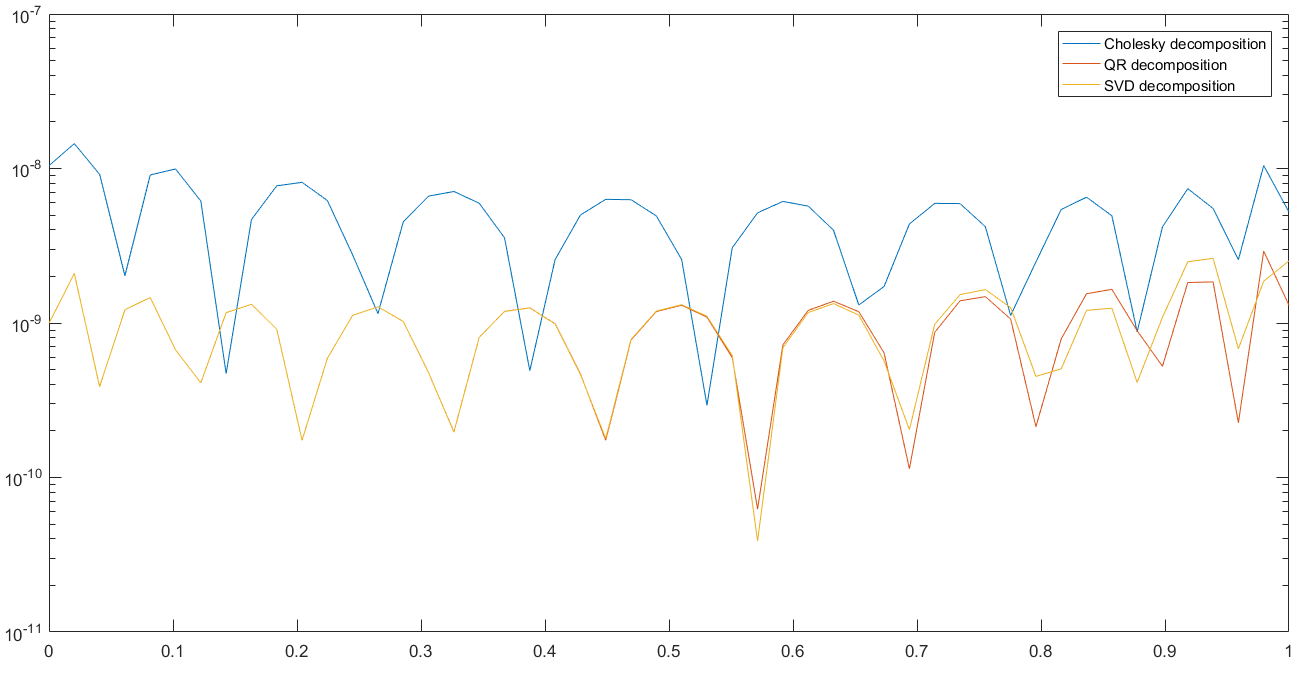
\includegraphics[width=1\textwidth]{residuals.png}
	\caption{\small Residuals computed for each of the coefficient vectors $\mathbf{c}^{(Chol)}$, $\mathbf{c}^{(QR)}$, and $\mathbf{c}^{(SVD)}$.}
\end{figure}
\noindent
\\\textbf{(f)} Print a table to 16 digits of precision showing the coefficients of the least-squares polynomials:

\begin{center}
	\begin{table}[h!]
		\centering
		\setlength\extrarowheight{6pt}
		\begin{tabular}{ |c|c|c|c| }
			\hline
			\textbf{n} & \textbf{Cholesky decomposition} & \textbf{QR decomposition} & \textbf{SVD decomposition} \\
			\hline
			0 & 0.999999989561589 & 1.000000000996608 & 1.000000000996610 \\
			\hline
			1 & 0.000002624202733 & -0.000000422743112 & -0.000000422743110 \\
			\hline
			2 & -8.000090615741891 & -7.999981235684255 & -7.999981235684690 \\
			\hline
			3 & 0.001236828943967 & -0.000318763244498 & -0.000318763245417 \\
			\hline
			4 & 10.657870472602468 & 10.669430795958332 & 10.669430795960118 \\
			\hline
			5 & \textcolor{red}{0.037032551084895} & -0.013820288155987 & -0.013820288089856 \\
			\hline
			6 & -5.788074905310304 & -5.647075627080019 & -5.647075626867935 \\
			\hline
			7 & \textcolor{red}{0.177871226754187} & -0.075316024565097 & -0.075316024316973 \\
			\hline
			8 & \textcolor{red}{1.399642921099546} & 1.693606963572196 & 1.693606963868704 \\
			\hline
			9 & \textcolor{red}{0.219057608697183} & 0.006032108788395 & 0.006032109701667 \\
			\hline
			10 & \textcolor{red}{-0.461840020342716} & -0.374241703484410 & -0.374241703992312 \\
			\hline
			11 & \textcolor{red}{0.103647702805936} & 0.088040576080084 & 0.088040576075623 \\
			\hline
		\end{tabular}
		\caption*{Coefficients of the least-squares polynomials using Cholesky, QR, \& SVD decomposition.}
	\end{table}
\end{center}
Highlighted coefficients are those from Cholesky decomposition, that are very different from QR and SVD decompositions.
\newpage
\section*{Question 3.}
\setcounter{equation}{0}
\textbf{(a)} Let $A \in \mathbb{C}^{n\times n} $ be an outer product of two vectors, i.e., $A=\mathbf{y}\mathbf{x}^H$ for some vectors $\mathbf{x},\mathbf{y}\in \mathbb{C}^n$. Show that $\norm{A}_2=\norm{\mathbf{x}}_2 \norm{\mathbf{y}}_2$, i.e., the (matrix) $\ell_2$-norm of $A$ is the product of the (vector) $\ell_2$-norm of $\mathbf{x}$ and $\mathbf{y}$.
\begin{margin}{0.5cm}{0.5cm}
	\begin{equation}
		AA^H = \mathbf{y}\mathbf{x}^H\mathbf{x}\mathbf{y}^H
	\end{equation}
	
	$\mathbf{x}$ is a vector in $\mathbb{C}^n \tab \Rightarrow \tab \mathbf{x}^H\mathbf{x} = \norm{\mathbf{x}}^2_2 \tab$
	
	\begin{equation}
		AA^H = \mathbf{y}\norm{\mathbf{x}}^2_2\mathbf{y}^H = \norm{\mathbf{x}}^2_2\mathbf{y}\mathbf{y}^H
	\end{equation}
	
	We define $\rho(B) := \max\{$\textit{absolute value of eigenvalues of B}$\}$
	
	\begin{equation}
		\sqrt{\rho(AA^H)} = \sqrt{\rho(\norm{\mathbf{x}}^2_2\mathbf{y}\mathbf{y}^H)}
	\end{equation}
	
	We know that:
	
	\begin{equation*}
		A\mathbf{v}=\lambda\mathbf{v}\ (\lambda \text{ eigenvalue of } A)\tab\Rightarrow\tab cA\mathbf{v}=c\lambda\mathbf{v}\	 (c\lambda \text{ eigenvalue of } cA\ \forall\ c\ \ne 0 \in\ \mathbb{R})
	\end{equation*}
	
	Equation (3) becomes:
	
	\begin{equation}
		\sqrt{\rho(AA^H)} = \sqrt{\norm{\mathbf{x}}^2_2\rho(\mathbf{y}\mathbf{y}^H)}
	\end{equation}
	
	Because $\norm{\mathbf{x}}_2 > 0$
	
	\begin{equation}
		\sqrt{\rho(AA^H)} = \norm{\mathbf{x}}_2\sqrt{\rho(\mathbf{y}\mathbf{y}^H)}
	\end{equation}
	
	Which by definition of $\ell_2$ norm becomes:
	
	\begin{equation}
		\norm{A}_2 = \norm{\mathbf{x}}_2\norm{\mathbf{y}}_2
	\end{equation}
	\\
\end{margin}
\textbf{(b)} Let $K_p(A)=\norm{A}_p\norm{A^{-1}}_p$ be the condition number of matrix inversion in the \textit{p}-norm. If $A \in \mathbb{C}^{n\times n}$ and $B \in \mathbb{C}^{n\times n}$ are both invertible, prove that $K_p(AB)\leq K_p(A)K_p(B)$.
\\
\setcounter{equation}{0}
\begin{margin}{0.5cm}{0.5cm}
	\textit{A} and \textit{B} are invertible then $AB \in \mathbb{C}^{n\times n}$ is invertible:
	\begin{equation}
		K_p(AB) = \norm{AB}_p\norm{(AB)^{-1}}_p = \norm{AB}_p\norm{B^{-1}A^{-1}}_p
	\end{equation}
	
	\textit{A} and \textit{B} are square matrices and all matrix \textit{p}-norms are consistent:
	
	\begin{equation*}
		\norm{AB} \leq \norm{A} \norm{B}
	\end{equation*}
	
	Equation (1) becomes:
	\begin{equation}
		K_p(AB) = \norm{AB}_p\norm{B^{-1}A^{-1}}_p \leq \norm{A} \norm{B} \norm{B^{-1}} \norm{A^{-1}}
	\end{equation}
	\begin{equation*}
		K_p(AB) \leq \norm{A} \norm{A^{-1}} \norm{B} \norm{B^{-1}}
	\end{equation*}
	
	\begin{equation*}
		K_p(AB) \leq K_p(A)K_p(B)
	\end{equation*}
	
\end{margin}

\section*{Question 4.}
The determinant of a triangular matrix is the product of its diagonal entries. Use this fact to develop a \textsc{Matlab} function \texttt{ludet} for computing the determinant of any arbitrary $A \in \mathbb{C}$ using its \textit{LU} decomposition.
\begin{margin}{0.5cm}{0.5cm}
	We implement \textit{LU} decomposition using \textsc{Matlab}'s \texttt{lu} command. The determinant is the product of the entries on the diagonal of the \textit{U} matrix.\\
	To determine the sign of the determinant, we count the number of permutations in the \textit{permutation} matrix returned by \texttt{lu} function. The following \textsc{Matlab} function shows the implementation:
\begin{lstlisting}[
style=Matlab-editor,
numbers=none,
frame=none,
xleftmargin=.2in
]
function d = ludet(A)
  [l, u, p] = lu(A);

  sign = 1;
  [row, col] = find(p);

  % counting the number of permutations
  for i=1:size(p)
    if(row(i) ~= i)
      j = find(row == i);  % other row index
      r = row(i);          % current row
      q = p(i,:);          % current permutation row

      row(i) = i;          % update current row
      p(i,:) = p(r,:);     % update current permutation row

      row(j) = r;          % update other row
      p(row(i),:) = q;     % update other permutation row

      sign = -sign;
    end
  end

  d = sign * prod(diag(u));
\end{lstlisting}
\noindent
\\\\The code is available as a \textsc{Matlab} file (\textit{ludet.m}) and a \textsc{Matlab} diary (\textit{ludet.txt})
\end{margin}

\end{document}
